\documentclass[12pt,a4paper]{article}
\usepackage[utf8]{inputenc}
\usepackage[vietnamese]{babel}
\usepackage{geometry}
\usepackage{graphicx}
\usepackage{amsmath}
\usepackage{amsfonts}
\usepackage{amssymb}
\usepackage{listings}
\usepackage{xcolor}
\usepackage{hyperref}
\usepackage{enumitem}
\usepackage{titlesec}
\usepackage{fancyhdr}
\usepackage{lastpage}
\usepackage{hyperref}
% Header configuration
\pagestyle{fancy}
\fancyhf{}
\fancyhead[L]{Chien Nguyen}
\fancyhead[R]{ \thepage\ }
\renewcommand{\headrulewidth}{0.4pt}

\geometry{margin=2.5cm}
\setlength{\parindent}{0pt}
\setlength{\parskip}{6pt}

% Code listing style
\lstset{
    basicstyle=\ttfamily\small,
    breaklines=true,
    frame=single,
    numbers=left,
    numberstyle=\tiny,
    keywordstyle=\color{blue},
    commentstyle=\color{green!60!black},
    stringstyle=\color{red},
    backgroundcolor=\color{gray!10}
}

% Title formatting
\titleformat{\section}{\Large\bfseries}{\thesection}{1em}{}
\titleformat{\subsection}{\large\bfseries}{\thesubsection}{1em}{}

\title{\textbf{BÁO CÁO THIẾT KẾ PAIN POINT TO SOLUTION AGENT}\\
\large Filum.ai AI Engineer Intern Assignment}
\author{Chien Nguyen}
\date{\today}

\documentclass[12pt,a4paper]{article}
\usepackage[utf8]{vietnam}
\usepackage{graphicx}
\usepackage{tikz}

\begin{document}

\begin{titlepage}
 \begin{tikzpicture}[remember picture, overlay]
 \draw[line width=1pt, blue!50!cyan]
 (current page.north west) rectangle (current page.south east);
 \end{tikzpicture}

 \centering
 \vspace*{2cm}

 % Logo công ty
 \includegraphics[width=0.8\textwidth]{logo.png}

 \vspace{2cm}

 % Tiêu đề
 {\Large \textbf{BÁO CÁO THIẾT KẾ }}
 \vspace{0.5cm}
 {\Large \textbf{\\PAIN POINT TO SOLUTION AGENT}}
 \vspace{0.5cm}

 {\large Filum.ai AI Engineer Intern Assignment}
\vspace{2cm}

{\large \textbf{Link GitHub } \href{https://github.com/chiennguyen/filum-agent}{Agentic RAG Pain point}}

 \vspace{5cm}

 % Thông tin ứng viên
 {\large \textbf{Ứng viên:} Nguyễn Tất Chiến}

 \vspace{0.5cm}

 {\large \textbf{Email:} Nguyentatchien9564@gmail.com}

 \vspace{0.5cm}

 {\large \textbf{Chức danh ứng tuyển:} AI Engineer Intern}

 \vfill

 % Ngày tháng
 {\large \today}
\end{titlepage}


\newpage

\tableofcontents
\newpage

\section{I. Tiếng Việt}

\subsection{Tổng quan}

Báo cáo này trình bày thiết kế và triển khai của một "Pain Point to Solution Agent" - một hệ thống AI được phát triển để phân tích các vấn đề kinh doanh và đề xuất các tính năng phù hợp từ nền tảng Filum.ai.

\subsection{KEY TASK}
\subsubsection{Định nghĩa Input của Agent}

\textbf{Yêu cầu}: Xác định thông tin cần thiết để agent hiểu hiệu quả pain point của user.

\textbf{Giải pháp triển khai}:
\begin{itemize}
    \item \textbf{Input Format}: Plain text với cấu trúc tự nhiên
    \item \textbf{Required Information}: Mô tả chi tiết vấn đề kinh doanh
    \item \textbf{Contextual Information}: 
    \begin{itemize}
        \item Loại hình doanh nghiệp (B2B/B2C)
        \item Quy mô công ty (Startup/SME/Enterprise)
        \item Ngành nghề (E-commerce/Service/Manufacturing)
    \end{itemize}
    \item \textbf{Validation}: Kiểm tra tính hợp lệ của câu hỏi business-related
\end{itemize}

\textbf{Ví dụ Input}:
\begin{lstlisting}[language=json, caption=Ví dụ Input Pain Point]
{
    "pain_point": "We're struggling to collect customer feedback consistently after a purchase",
    "business_context": {
        "business_type": "B2C",
        "company_size": "SME",
        "industry": "E-commerce"
    },
    "additional_context": "Online retail store with 1000+ monthly orders"
}
\end{lstlisting}
\newpage
\subsubsection{ Output của Agent}

\textbf{Yêu cầu}: Cách thức trình bày các giải pháp Filum.ai được đề xuất.

\textbf{Giải pháp triển khai}:
\begin{itemize}
    \item \textbf{Output Structure}: JSON format với các trường:
    \begin{itemize}
        \item \texttt{feature\_name}: Tên tính năng
        \item \texttt{how\_it\_helps}: Mô tả cách giải quyết vấn đề
        \item \texttt{relevance\_score}: Điểm đánh giá độ liên quan (0-1)
        \item \texttt{link\_to\_info}: Liên kết thông tin chi tiết
    \end{itemize}
    \item \textbf{Multiple Solutions}: Hỗ trợ đề xuất nhiều giải pháp
    \item \textbf{Actionable Information}: Thông tin có thể thực hiện ngay
\end{itemize}

\textbf{Ví dụ Output}:
\begin{lstlisting}[language=json, caption=Ví dụ Output Solutions]
{
    "suggested_solutions": [
        {
            "feature_name": "Automated Post-Purchase Surveys",
            "how_it_helps": "Trigger surveys automatically via email/SMS after a transaction to collect consistent customer feedback",
            "relevance_score": 0.85,
            "link_to_info": "https://filum.ai/voc/surveys",
            "category": "VoC - Surveys"
        },
        {
            "feature_name": "Customer Journey Analytics",
            "how_it_helps": "Track customer touchpoints and identify feedback collection opportunities",
            "relevance_score": 0.72,
            "link_to_info": "https://filum.ai/insights/experience",
            "category": "Insights - Experience"
        }
    ],
    "analysis_summary": {
        "total_problems": 1,
        "total_outcomes": 1,
        "resolved_count": 2,
        "search_iterations": 1,
        "overall_status": "resolved"
    }
}
\end{lstlisting}

\subsubsection{ Thiết kế Feature Knowledge Base Structure}

\textbf{Yêu cầu}: Cách biểu diễn features và capabilities của Filum.ai.

\textbf{Giải pháp triển khai}:
\begin{itemize}
    \item \textbf{Data Structure}: JSON schema với các thuộc tính:
    \begin{itemize}
        \item \texttt{feature\_id}: Định danh duy nhất
        \item \texttt{feature\_name}: Tên tính năng
        \item \texttt{description}: Mô tả chi tiết
        \item \texttt{keywords}: Từ khóa tìm kiếm
        \item \texttt{pain\_points\_solved}: Các vấn đề được giải quyết
        \item \texttt{link}: Liên kết thông tin
    \end{itemize}
    \item \textbf{Vector Embeddings}: Sử dụng semantic search
    \item \textbf{Metadata}: Thông tin bổ sung cho matching algorithm
\end{itemize}

\textbf{Ví dụ Feature Database Entry}:
\begin{lstlisting}[language=json, caption=Ví dụ Feature Database Schema]
{
    "feature_id": "voc_surveys_001",
    "feature_name": "Automated Post-Purchase Surveys",
    "description": "Automatically trigger customer feedback surveys after purchase transactions via email, SMS, or in-app notifications",
    "keywords": ["feedback", "survey", "post-purchase", "customer", "automation", "email", "sms"],
    "pain_points_solved": [
        "inconsistent feedback collection",
        "manual survey distribution",
        "low response rates",
        "delayed feedback collection"
    ],
    "category": "VoC - Surveys",
    "link": "https://filum.ai/voc/surveys",
    "metadata": {
        "business_type": ["B2C", "B2B"],
        "company_size": ["Startup", "SME", "Enterprise"],
        "industry": ["E-commerce", "Retail", "Service"]
    }
}
\end{lstlisting}

\subsection{System Architecture (Vietnamese)}

\begin{figure}[h]
    \centering
    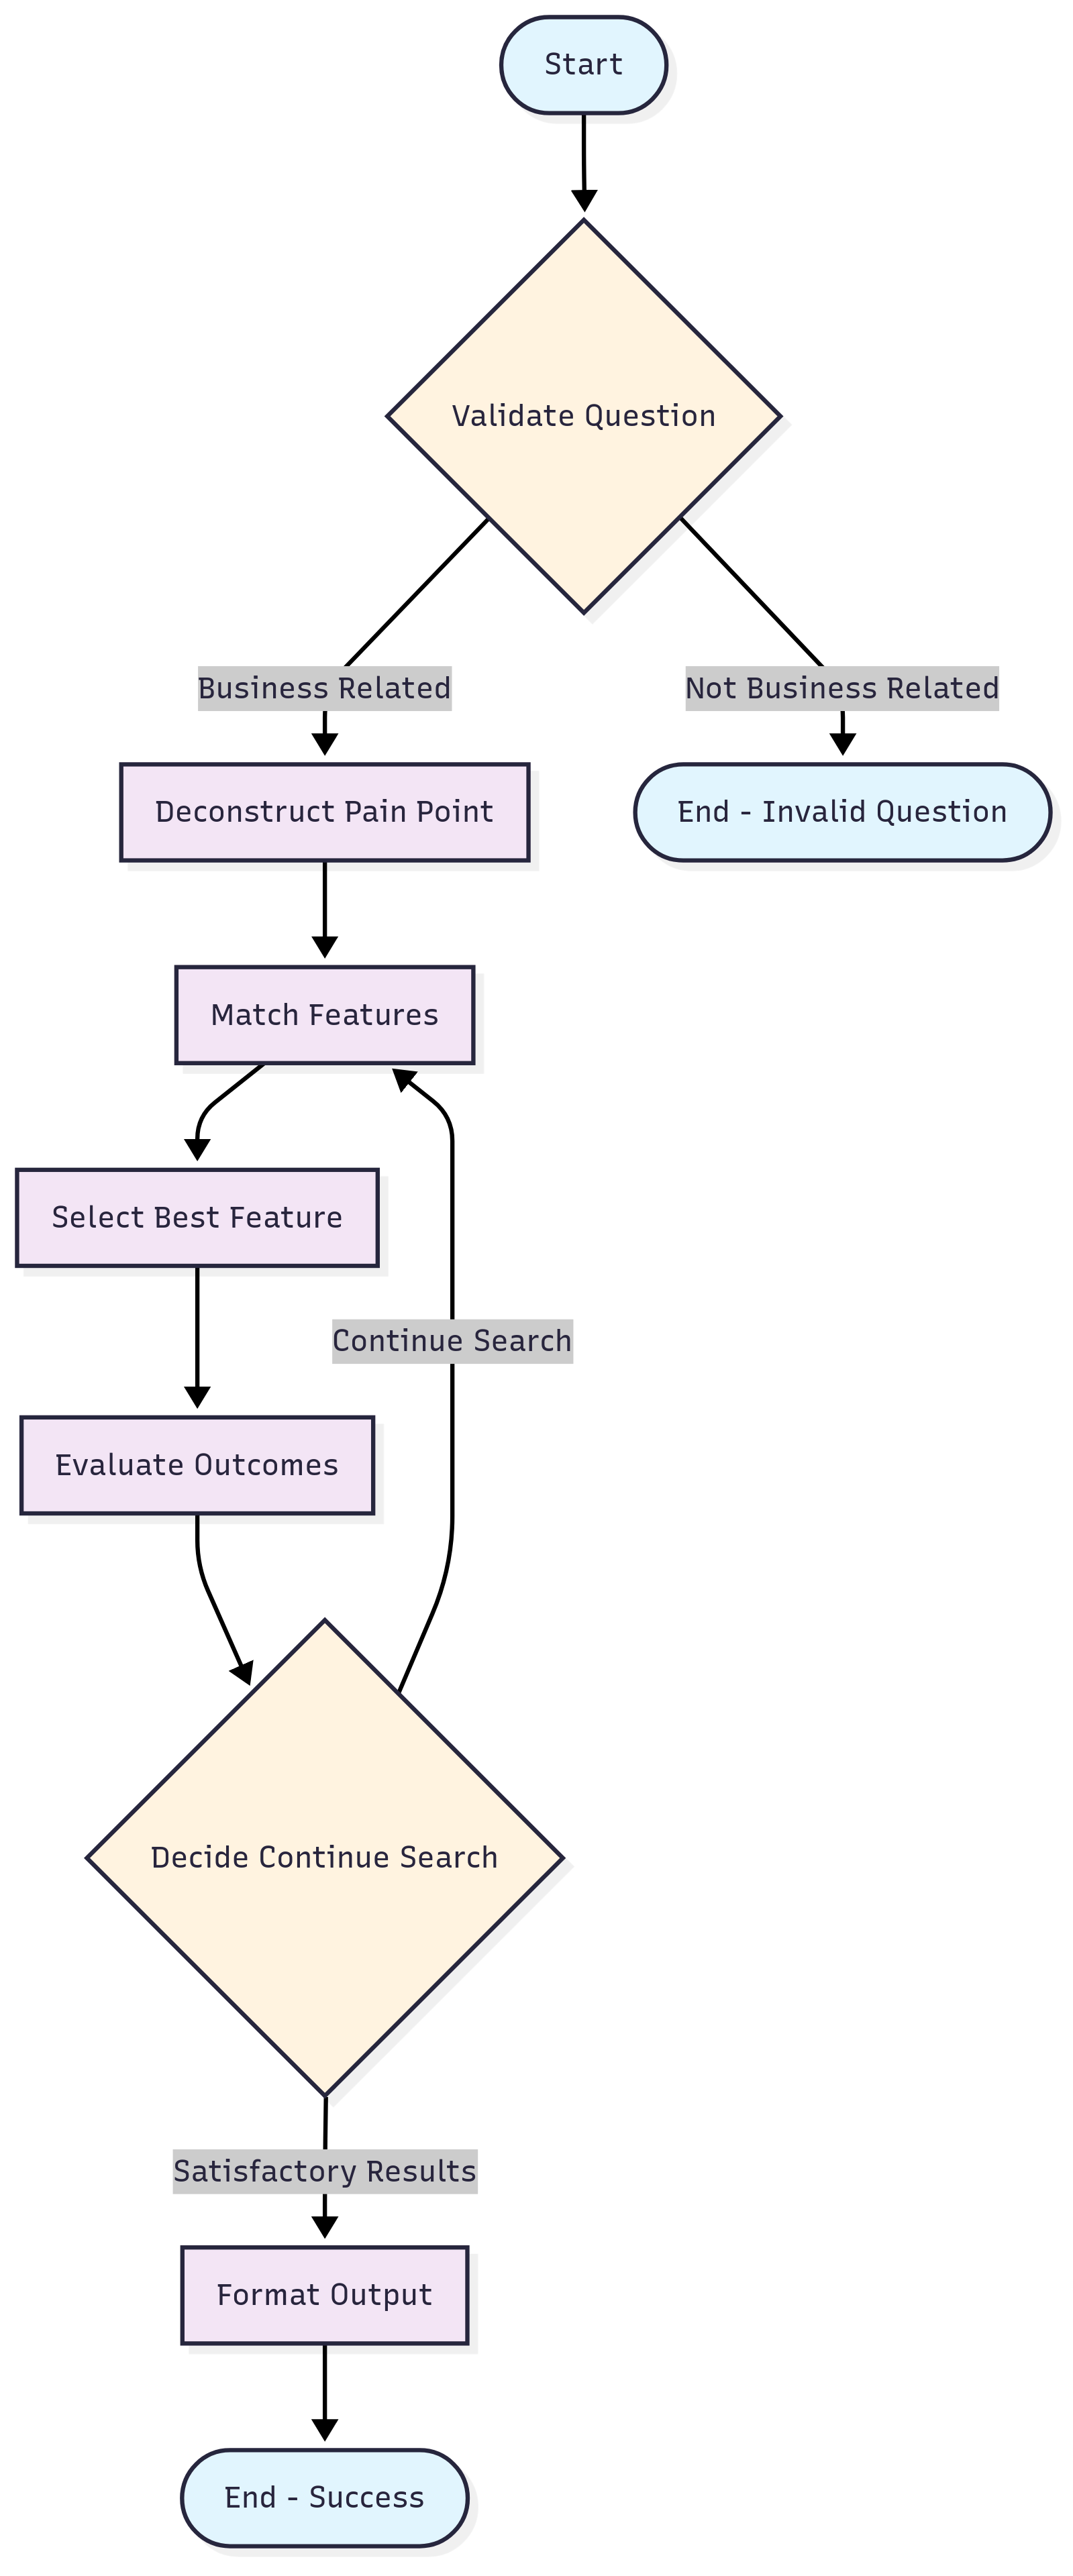
\includegraphics[width=0.3\textwidth]{Flow.png}
    \caption{Workflow của Pain Point to Solution Agent}
    \label{fig:workflow}
\end{figure}
\newpage
\subsubsection{Workflow chính}
Hệ thống được thiết kế theo mô hình ReAct (Reasoning and Acting) với các bước chính:

\begin{enumerate}[label=\textbf{\arabic*.}]
    \item \textbf{Validate Question}: Kiểm tra tính hợp lệ của câu hỏi
    \item \textbf{Deconstruct Pain Point}: Phân tích vấn đề thành các thành phần nhỏ
    \item \textbf{Match Features}: Tìm kiếm tính năng phù hợp
    \item \textbf{Select Best Feature}: Chọn tính năng tốt nhất
    \item \textbf{Evaluate Outcomes}: Đánh giá hiệu quả
    \item \textbf{Decide Continue Search}: Quyết định có tiếp tục tìm kiếm không
    \item \textbf{Format Output}: Định dạng kết quả cuối cùng
\end{enumerate}

Như thể hiện trong Hình~\ref{fig:workflow}, hệ thống bắt đầu với việc validate câu hỏi, sau đó thực hiện quy trình iterative cho đến khi đạt được kết quả thỏa mãn.

\subsubsection{Cấu trúc dữ liệu}

\begin{lstlisting}[language=Python, caption=Cấu trúc AgentState]
class AgentState(TypedDict):
    pain_point: str
    deconstructed: Optional[Dict[str, List[str]]]
    best_feature: Optional[Dict[str, str]]
    selected_features: List[Dict[str, Any]]
    evaluation_results: Optional[Dict[str, Any]]
    should_continue_search: bool
    search_iteration: int
    final_output: Optional[Dict[str, Any]]
\end{lstlisting}

\subsection{Vector Search Implementation}

Sử dụng ChromaDB với Google Generative AI Embeddings để tìm kiếm semantic:

\begin{lstlisting}[language=Python, caption=Vector Store Setup]
def setup_vector_store(self):
    embedding_model = GoogleGenerativeAIEmbeddings(
        model="models/text-embedding-004"
    )
    self.vector_store = Chroma.from_documents(
        documents=documents,
        embedding=embedding_model,
        persist_directory="./chroma_db"
    )
\end{lstlisting}

\subsection{Thuật toán Matching}

\subsubsection{Deconstruction Process}

Hệ thống phân tích pain point thành hai thành phần chính:

\begin{itemize}
    \item \textbf{Current Problems}: Các vấn đề hiện tại
    \item \textbf{Desired Outcomes}: Kết quả mong muốn
\end{itemize}

\subsubsection{Feature Selection Logic}

Sử dụng LLM để đánh giá và chọn tính năng phù hợp nhất dựa trên:

\begin{itemize}
    \item Độ liên quan (relevance score)
    \item Khả năng giải quyết vấn đề
    \item Hiệu quả đạt được kết quả mong muốn
\end{itemize}

\subsection{Kết quả thử nghiệm}

\subsubsection{Ví dụ test case}

\textbf{Input}: "We're struggling to collect customer feedback consistently after a purchase"

\textbf{Output}: 
\begin{itemize}
    \item \textbf{Automated Post-Purchase Surveys} (VoC - Surveys)
    \item \textbf{Relevance Score}: 0.85
    \item \textbf{How it helps}: Trigger surveys automatically via email/SMS after a transaction
\end{itemize}

\subsection{Kết luận}

Hệ thống Pain Point to Solution Agent đã được thiết kế với:

\begin{itemize}
    \item Kiến trúc modular và scalable
    \item Output có cấu trúc rõ ràng và actionable
\end{itemize}

Hệ thống có thể được mở rộng để hỗ trợ thêm các loại tính năng validate input , hệ thống phòng vệ và cải thiện độ chính xác của matching algorithm.

\section{II. Tiếng Anh}

\subsection{Overview}

This report presents the design and implementation of a "Pain Point to Solution Agent" - an AI system developed to analyze business problems and suggest relevant features from the Filum.ai platform.

\subsection{KEY TASK}
\subsubsection{Define Agent Input}

\textbf{Requirement}: Determine the information needed for the agent to effectively understand user pain points.

\textbf{Implementation Solution}:
\begin{itemize}
    \item \textbf{Input Format}: Plain text with natural structure
    \item \textbf{Required Information}: Detailed description of business problems
    \item \textbf{Contextual Information}: 
    \begin{itemize}
        \item Business type (B2B/B2C)
        \item Company size (Startup/SME/Enterprise)
        \item Industry (E-commerce/Service/Manufacturing)
    \end{itemize}
    \item \textbf{Validation}: Check validity of business-related questions
\end{itemize}

\textbf{Input Example}:
\begin{lstlisting}[language=json, caption=Input Pain Point Example]
{
    "pain_point": "We're struggling to collect customer feedback consistently after a purchase",
    "business_context": {
        "business_type": "B2C",
        "company_size": "SME",
        "industry": "E-commerce"
    },
    "additional_context": "Online retail store with 1000+ monthly orders"
}
\end{lstlisting}

\newpage
\subsubsection{Agent Output}

\textbf{Requirement}: How to present suggested Filum.ai solutions.

\textbf{Implementation Solution}:
\begin{itemize}
    \item \textbf{Output Structure}: JSON format with fields:
    \begin{itemize}
        \item \texttt{feature\_name}: Feature name
        \item \texttt{how\_it\_helps}: Description of how it solves the problem
        \item \texttt{relevance\_score}: Relevance rating (0-1)
        \item \texttt{link\_to\_info}: Detailed information link
    \end{itemize}
    \item \textbf{Multiple Solutions}: Support for suggesting multiple solutions
    \item \textbf{Actionable Information}: Information that can be implemented immediately
\end{itemize}

\textbf{Output Example}:
\begin{lstlisting}[language=json, caption=Output Solutions Example]
{
    "suggested_solutions": [
        {
            "feature_name": "Automated Post-Purchase Surveys",
            "how_it_helps": "Trigger surveys automatically via email/SMS after a transaction to collect consistent customer feedback",
            "relevance_score": 0.85,
            "link_to_info": "https://filum.ai/voc/surveys",
            "category": "VoC - Surveys"
        },
        {
            "feature_name": "Customer Journey Analytics",
            "how_it_helps": "Track customer touchpoints and identify feedback collection opportunities",
            "relevance_score": 0.72,
            "link_to_info": "https://filum.ai/insights/experience",
            "category": "Insights - Experience"
        }
    ],
    "analysis_summary": {
        "total_problems": 1,
        "total_outcomes": 1,
        "resolved_count": 2,
        "search_iterations": 1,
        "overall_status": "resolved"
    }
}
\end{lstlisting}

\subsubsection{Feature Knowledge Base Structure Design}

\textbf{Requirement}: How to represent Filum.ai features and capabilities.

\textbf{Implementation Solution}:
\begin{itemize}
    \item \textbf{Data Structure}: JSON schema with attributes:
    \begin{itemize}
        \item \texttt{feature\_id}: Unique identifier
        \item \texttt{feature\_name}: Feature name
        \item \texttt{description}: Detailed description
        \item \texttt{keywords}: Search keywords
        \item \texttt{pain\_points\_solved}: Problems solved
        \item \texttt{link}: Information link
    \end{itemize}
    \item \textbf{Vector Embeddings}: Using semantic search
    \item \textbf{Metadata}: Additional information for matching algorithm
\end{itemize}

\textbf{Feature Database Entry Example}:
\begin{lstlisting}[language=json, caption=Feature Database Schema Example]
{
    "feature_id": "voc_surveys_001",
    "feature_name": "Automated Post-Purchase Surveys",
    "description": "Automatically trigger customer feedback surveys after purchase transactions via email, SMS, or in-app notifications",
    "keywords": ["feedback", "survey", "post-purchase", "customer", "automation", "email", "sms"],
    "pain_points_solved": [
        "inconsistent feedback collection",
        "manual survey distribution",
        "low response rates",
        "delayed feedback collection"
    ],
    "category": "VoC - Surveys",
    "link": "https://filum.ai/voc/surveys",
    "metadata": {
        "business_type": ["B2C", "B2B"],
        "company_size": ["Startup", "SME", "Enterprise"],
        "industry": ["E-commerce", "Retail", "Service"]
    }
}
\end{lstlisting}

\subsection{System Architecture (English)}

\begin{figure}[h]
    \centering
    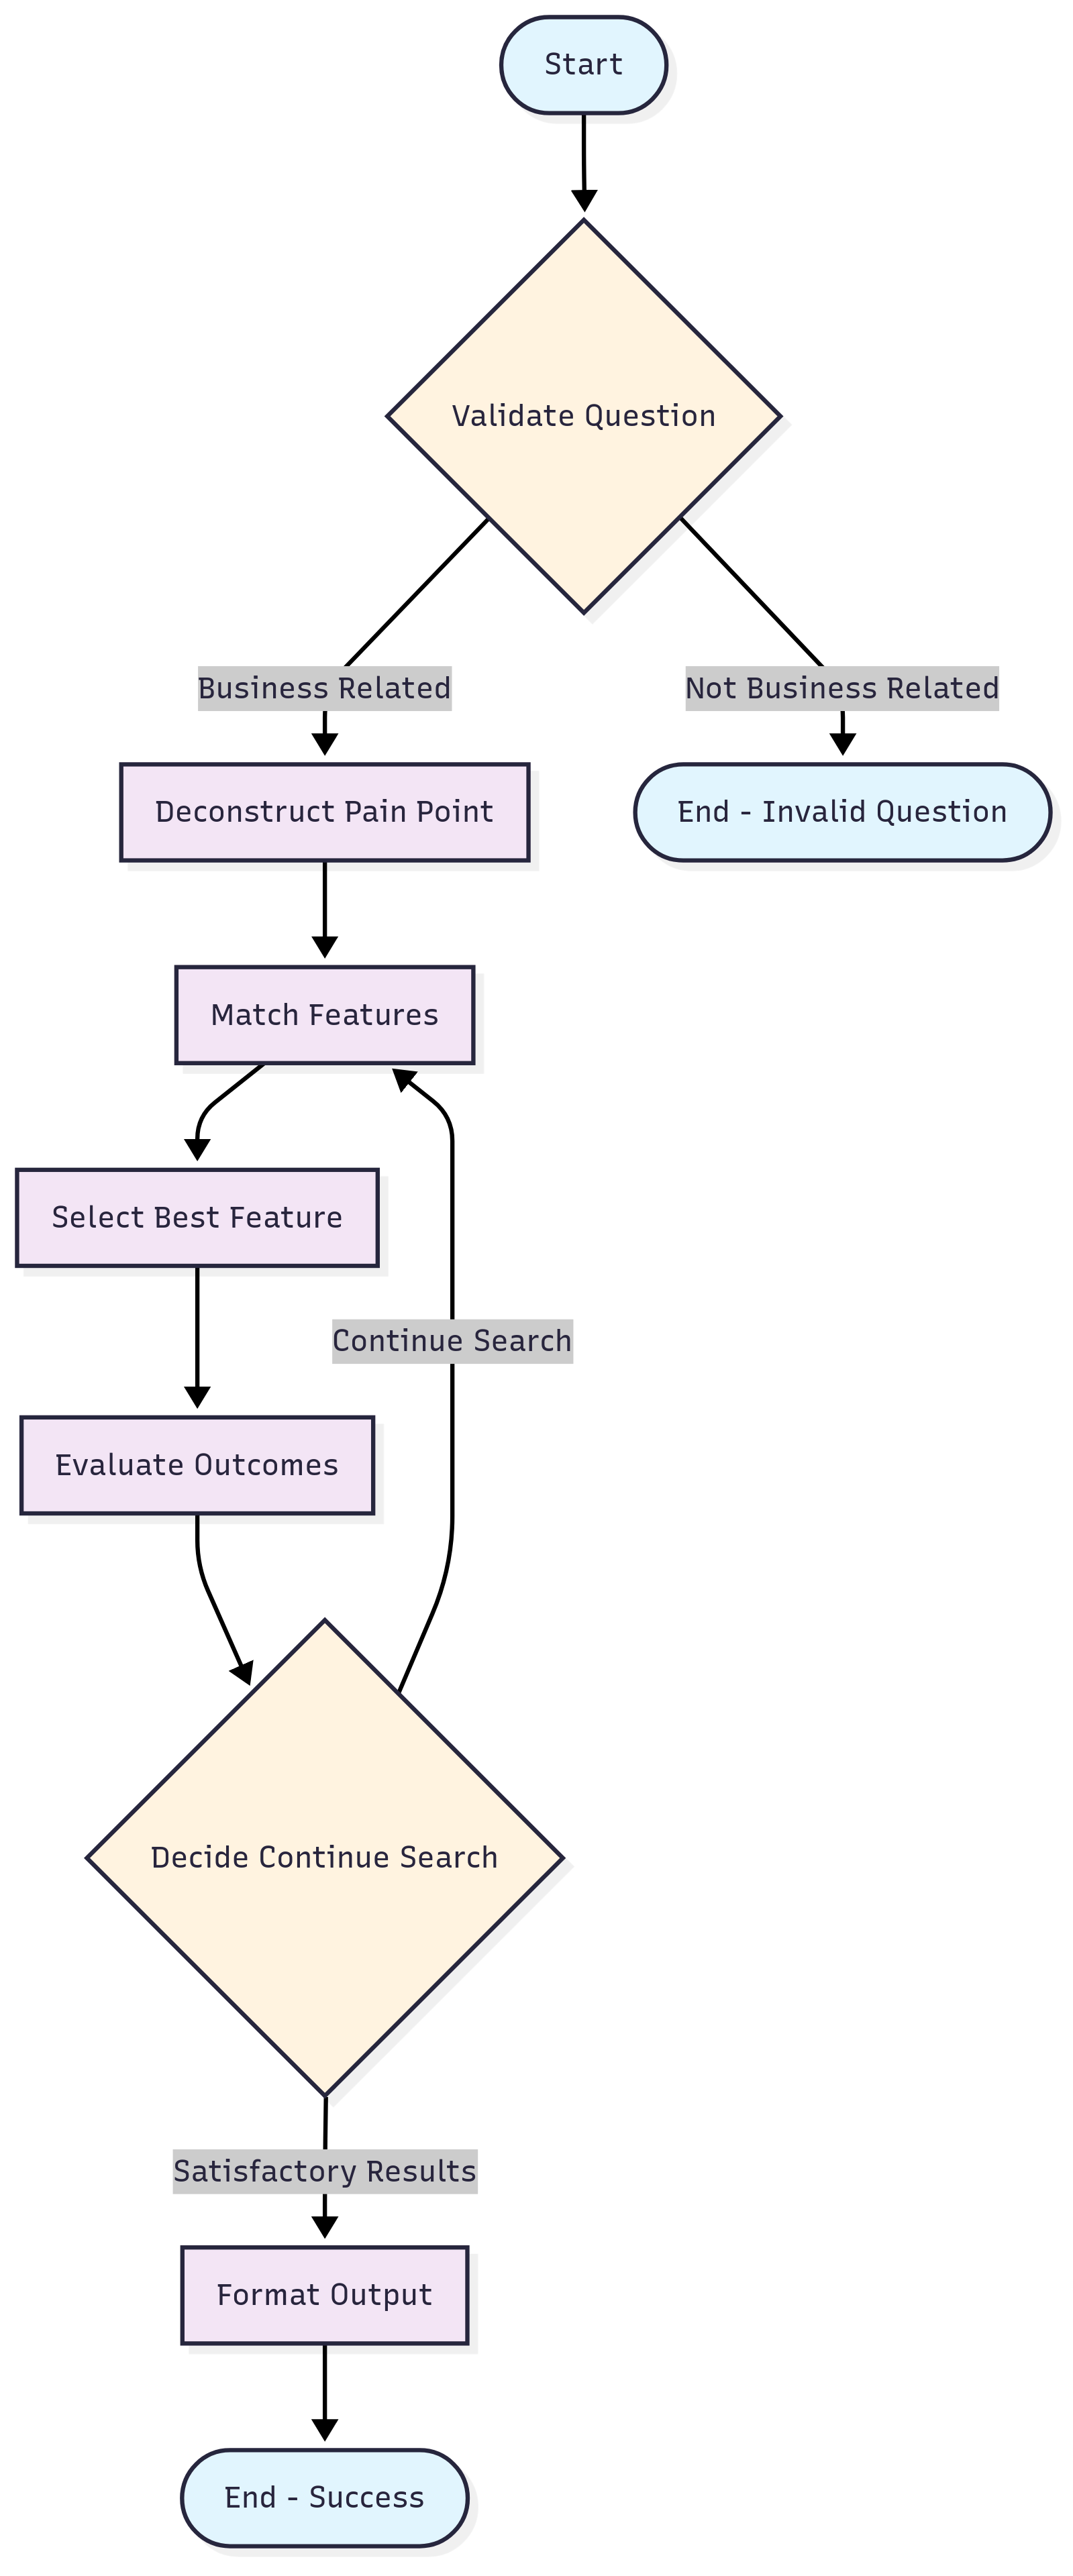
\includegraphics[width=0.3\textwidth]{Flow.png}
    \caption{Workflow of Pain Point to Solution Agent}
    \label{fig:workflow-en}
\end{figure}
\newpage
\subsubsection{Main Workflow}
The system is designed following the ReAct (Reasoning and Acting) model with the following main steps:

\begin{enumerate}[label=\textbf{\arabic*.}]
    \item \textbf{Validate Question}: Check the validity of the question
    \item \textbf{Deconstruct Pain Point}: Analyze the problem into smaller components
    \item \textbf{Match Features}: Search for suitable features
    \item \textbf{Select Best Feature}: Choose the best feature
    \item \textbf{Evaluate Outcomes}: Assess effectiveness
    \item \textbf{Decide Continue Search}: Decide whether to continue searching
    \item \textbf{Format Output}: Format the final result
\end{enumerate}

As shown in Figure~\ref{fig:workflow-en}, the system starts with question validation, then performs an iterative process until satisfactory results are achieved.

\subsubsection{Data Structure}

\begin{lstlisting}[language=Python, caption=AgentState Structure]
class AgentState(TypedDict):
    pain_point: str
    deconstructed: Optional[Dict[str, List[str]]]
    best_feature: Optional[Dict[str, str]]
    selected_features: List[Dict[str, Any]]
    evaluation_results: Optional[Dict[str, Any]]
    should_continue_search: bool
    search_iteration: int
    final_output: Optional[Dict[str, Any]]
\end{lstlisting}

\subsection{Vector Search Implementation}

Using ChromaDB with Google Generative AI Embeddings for semantic search:

\begin{lstlisting}[language=Python, caption=Vector Store Setup]
def setup_vector_store(self):
    embedding_model = GoogleGenerativeAIEmbeddings(
        model="models/text-embedding-004"
    )
    self.vector_store = Chroma.from_documents(
        documents=documents,
        embedding=embedding_model,
        persist_directory="./chroma_db"
    )
\end{lstlisting}

\subsection{Matching Algorithm}

\subsubsection{Deconstruction Process}

The system analyzes pain points into two main components:

\begin{itemize}
    \item \textbf{Current Problems}: Current issues
    \item \textbf{Desired Outcomes}: Desired results
\end{itemize}

\subsubsection{Feature Selection Logic}

Using LLM to evaluate and select the most suitable feature based on:

\begin{itemize}
    \item Relevance score
    \item Problem-solving capability
    \item Effectiveness in achieving desired outcomes
\end{itemize}

\subsection{Test Results}

\subsubsection{Test Case Example}

\textbf{Input}: "We're struggling to collect customer feedback consistently after a purchase"

\textbf{Output}: 
\begin{itemize}
    \item \textbf{Automated Post-Purchase Surveys} (VoC - Surveys)
    \item \textbf{Relevance Score}: 0.85
    \item \textbf{How it helps}: Trigger surveys automatically via email/SMS after a transaction
\end{itemize}

\subsection{Conclusion}

The Pain Point to Solution Agent system has been designed with:

\begin{itemize}
    \item Modular and scalable architecture
    \item Clear and actionable output structure
\end{itemize}

The system can be extended to support additional feature types, input validation, defense systems, and improve the accuracy of the matching algorithm.

\end{document}
